%%!TEX root=../main.tex

\section{Evaluation}
We now analysis the performance of our various methods on different inputs. 
For CNN, we separately use original data and sparse representing data as our inputs.
For SVM, we only use sparse representing data as our inputs. 
We will mainly focus on the validation accuracy to evaluate different methods.

\subsection{CNN based method}
\textbf{Letter and Area} 
For letter and area, we use the same network architecture to train both original data and sparse data.
Figure \ref{letter} shows the training performance on original data and sparse data. 
The running time and training accuracy are shown in table \ref{label1}. 
From the table, we can see the final accuracy on test, train or validation set are mostly the same.
We can also see that the rates of convergence are different. 
For the original data, the network only need 10 epochs to converge 
whereas the network of sparse data converge after 175 epochs.

\begin{figure}[ht]
\centering
\subfloat{
    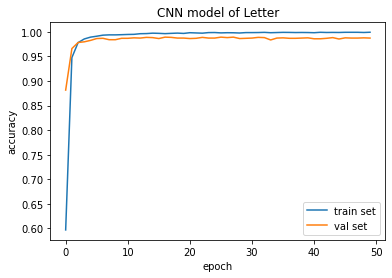
\includegraphics[width=1.4in]{\FIGDIR/letter_acc_original.png}
}
\qquad
\subfloat{
    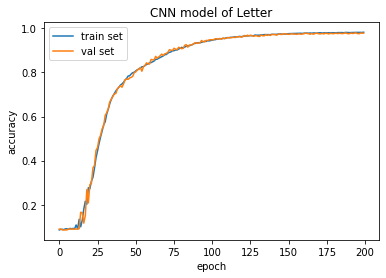
\includegraphics[width=1.4in]{\FIGDIR/letter_acc_s.png}
}
\qquad
\subfloat{
    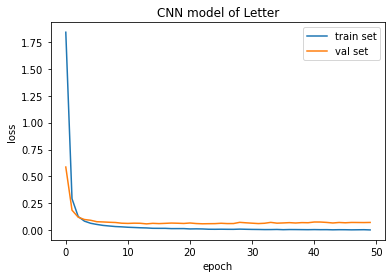
\includegraphics[width=1.4in]{\FIGDIR/letter_loss_original.png}
}
\qquad
\subfloat{
    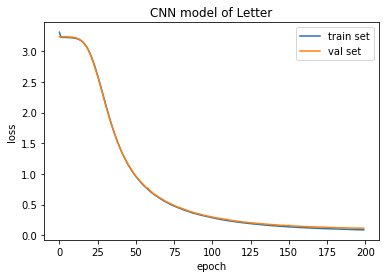
\includegraphics[width=1.4in]{\FIGDIR/letter_loss_s.png}
}
\qquad
\subfloat{
    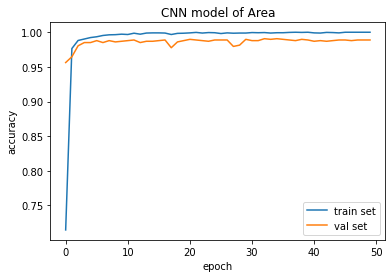
\includegraphics[width=1.4in]{\FIGDIR/area_acc_original.png}
}
\qquad
\subfloat{
    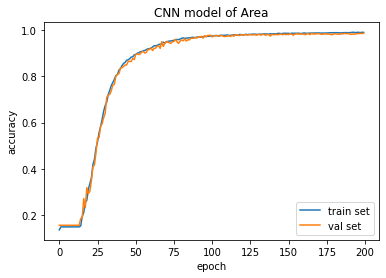
\includegraphics[width=1.4in]{\FIGDIR/area_acc_s.png}
}
\qquad
\subfloat{
    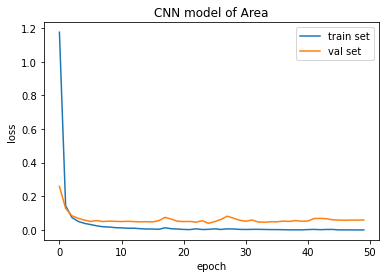
\includegraphics[width=1.4in]{\FIGDIR/area_loss_original.png}
}
\qquad
\subfloat{
    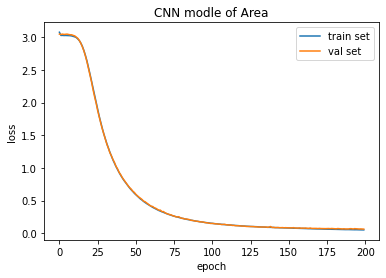
\includegraphics[width=1.4in]{\FIGDIR/area_loss_s.png}
}
\qquad
\caption{The right side shows the performance on original data, the left side shows the performance on sparse data}
\label{letter}
\end{figure}

\begin{table}[ht]
\centering
\scalebox{0.70} {
    \begin{tabular}{|c|c|c|c|c|}
        \hline
        Method&Prediction time&Train accuracy&Validation accuracy&Test accuracy\\
        \hline
        Letter (Sparse)&249ms&0.9824&0.9782&0.9772\\
        \hline
        Letter (Original)&166ms&0.9991&0.9872&0.9905\\
        \hline
        Area (Sparse)&126ms&0.9886&0.9851&0.9851\\
        \hline
        Area (Original)&126ms&0.9988&0.9879&0.9910\\
        \hline
    \end{tabular}
}
\caption{Running time and accuracy on letter and area category}
\label{label1}
\end{table}

\textbf{Province} 
For the data of province, we use different architectures on different data set. 
Figure \ref{provicne} shows the training performance using different input set. 
Table \ref{label2} shows the running time and accuracy. 
The difference between the original images and sparse representation is 
much more than the category of area and letter. 
Firstly, original images could reach 97.48\% whereas the sparse data could 
only reach 87.74\% on validation set. 
That could be explained that the architecture of network trained using the 
original images are similar to VGG16 being is a deep convolution network.
As for sparse data, it has two convolution network which is a lot shallower. 
In addition, we can find the network of sparse data is over-fitting, 
although we have tried multiple ways to avoid over-fitting 
such as adding drop layer, reducing the depth, it still exists. 

Also, in the terms of running time, the sparse data model takes less time 
than the original data model meaning the sparse representation can 
reduce the running time to some extent. 

\begin{figure}[ht]
\centering
\subfloat{
    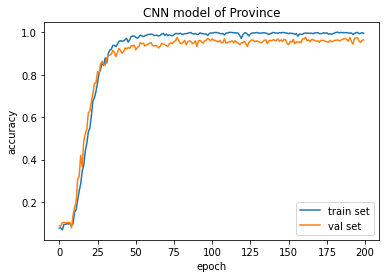
\includegraphics[width=1.45in]{\FIGDIR/province_acc_original.png}
}
\qquad
\subfloat{
    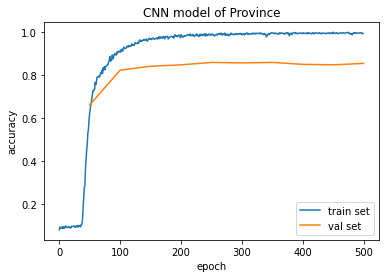
\includegraphics[width=1.45in]{\FIGDIR/province_acc_s.png}
}
\qquad
\subfloat{
    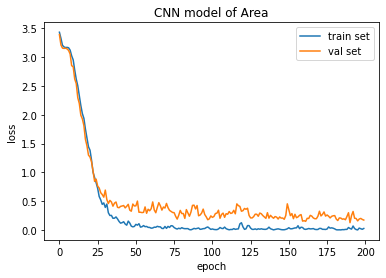
\includegraphics[width=1.45in]{\FIGDIR/province_loss_original.png}
}
\qquad
\subfloat{
    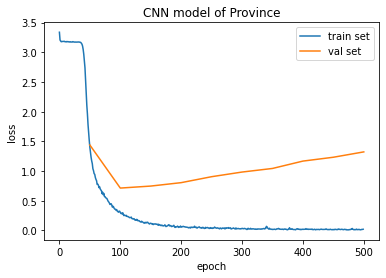
\includegraphics[width=1.45in]{\FIGDIR/province_loss_s.png}
}
\qquad
\caption{The right side shows the performance on original data, the left side shows the performance on sparse data}
\label{provicne}
\end{figure}

\begin{table}[ht]
\centering
\scalebox{0.70} {
    \begin{tabular}{|c|c|c|c|c|}
        \hline
        Method&Prediction time&Train accuracy&Validation accuracy&Test accuracy\\
        \hline
        Province (Sparse)&72ms&0.9927&0.8539&0.8774\\
        \hline
        Province (Original)&108ms&0.9949&0.9640&0.9748\\
        \hline
    \end{tabular}
}
\caption{Running time and accuracy on province category}
\label{label2}
\end{table}

\subsection{SVM Based method}
For SVM method, we only use sparse data to investigate the performance. 
The result and performance are shown in table \ref{tabel3}. 
From the table we can find compared with CNN method, the test accuracy 
is very similar, however the running time is different. 
SVM takes less time to train the model whereas more time on prediction.

\begin{table}[ht]
\centering
\scalebox{0.80} {
    \begin{tabular}{|c|c|c|c|}
        \hline
        Category&Training time&Prediction time&Testing accuracy\\
        \hline
        Letter &24.04s&6.17s&0.981\\
        \hline
        Area&7.67s&1.51s&0.9784\\
        \hline
        Province&4.07s&0.45s&0.875\\
        \hline
    \end{tabular}
}
\caption{Running time and accuracy on different inputs of province}
\label{tabel3}
\end{table}

